\documentclass[12pt, oneside]{article}
\usepackage[letterpaper, margin=1in, headsep=0.5in]{geometry}
\usepackage[english]{babel}
\usepackage[utf8]{inputenc}
\usepackage{amsmath}
\usepackage{amsfonts}
\usepackage{amssymb}
\usepackage{tikz}
\usetikzlibrary{quotes, angles}
\usepackage{graphicx}
%\usepackage{pgfplots}
%\pgfplotsset{width=10cm,compat=1.9}
%\usepgfplotslibrary{statistics}
%\usepackage{pgfplotstable}
%\usepackage{tkz-fct}
%\usepackage{venndiagram}

\usepackage{fancyhdr}
\pagestyle{fancy}
\fancyhf{}
\rhead{\thepage \\Name: \hspace{1.5in}.\\}
\lhead{BECA / Dr. Huson / Geometry 10th Grade\\* Unit 1: Introduction to Geometry\\
9 Sept 2019}

\renewcommand{\headrulewidth}{0pt}

\begin{document}
\subsubsection*{Homework 1.3: Equilateral triangle construction}
  \vspace{0.5cm}
  \begin{enumerate}

    \item Construct an equilateral triangle with $\overline{AB}$ as one side. Use a compass and straightedge. \vspace{5cm}
    \begin{center}
    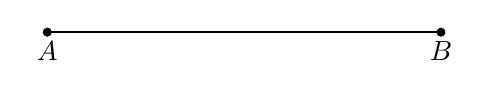
\begin{tikzpicture}[scale=1]
      \draw [-, thick] (0,0)--(5,0);
      \draw [fill] (0,0) circle [radius=0.05] node[below]{$A$};
      \draw [fill] (5,0) circle [radius=0.05] node[below]{$B$};
    \end{tikzpicture}
    \end{center}  \vspace{3cm}

    \item Write down the name of the angle shown in the diagram below using proper geometric notation.
    \begin{center}
    \begin{tikzpicture}[scale=2]
      \draw [->, thick] (0,0)--(4,3);
      \draw [->, thick] (0,0)--(5,-1);
      \draw [fill] (2.66666,2) circle [radius=0.025] node[above left ]{$D$};
      \draw [fill] (0,0) circle [radius=0.025] node[above left]{$E$};
      \draw [fill] (4,-0.8) circle [radius=0.025] node[above]{$F$};
    \end{tikzpicture}
    \end{center}
    Find the measure of the angle in degrees with a protractor.
    
  \newpage
    \item The points where a line segment begins and ends are the $\rule{4cm}{0.15mm}$. \bigskip
    \item A(n) $\rule{4cm}{0.15mm}$ is a portion of a line that includes two points and all of the collinear points between the two points.\bigskip
    \item A(n) $\rule{4cm}{0.15mm}$ is a portion of a line that begins with a single point and extends infinitely in one direction.
    \item Points that are all located on the same line are $\rule{4cm}{0.15mm}$.\bigskip
    \item Two or more line segments of equal measure are $\rule{4cm}{0.15mm}$.\bigskip
    \item A flat surface is a(n) $\rule{4cm}{0.15mm}$. \bigskip
    \item A(n) $\rule{4cm}{0.15mm}$ is a straight continuous arrangement of an infinite number of points.
    \bigskip
  \item Use symbols to write the name of each geometric figure.
  \begin{enumerate}
  \item %Ray DE
    \begin{tikzpicture}
      \draw [->, thick] (0,0)--(3,1.5);
      \draw [fill] (0,0) circle [radius=0.05] node[below]{$D$};
      \draw [fill] (2,1) circle [radius=0.05] node[below]{$E$};
    \end{tikzpicture} \bigskip
  \item \hspace{1cm}%Line AB
    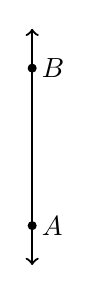
\begin{tikzpicture}
      \draw [<->, thick] (1,0)--(1,3);
      \draw [fill] (1,0.5) circle [radius=0.05] node[right]{$A$};
      \draw [fill] (1,2.5) circle [radius=0.05] node[right]{$B$};
    \end{tikzpicture} \bigskip
    \item %Line segment XY
      \begin{tikzpicture}
        \draw [-, thick] (1,0)--(0,2);
        \draw [fill] (1,0) circle [radius=0.05] node[below]{$X$};
        \draw [fill] (0,2) circle [radius=0.05] node[left]{$Y$};
      \end{tikzpicture}
  \end{enumerate}

\end{enumerate}
\end{document}
